% Created 2026-05-26 Tue 23:23
% Intended LaTeX compiler: pdflatex
\documentclass[11pt]{article}
\usepackage[utf8]{inputenc}
\usepackage[T1]{fontenc}
\usepackage[activate={true,nocompatibility},final,tracking=true,kerning=true,spacing=true,factor=1100,stretch=10,shrink=10]{microtype}
\usepackage[dvipsnames,svgnames]{xcolor}
\usepackage{hyperref}
\usepackage[utf8]{inputenc}
\usepackage{fixltx2e}
\usepackage{graphicx}
\usepackage{longtable}
\usepackage{float}
\usepackage{wrapfig}
\usepackage{rotating}
\usepackage[normalem]{ulem}
\usepackage{amsmath}
\usepackage{textcomp}
\usepackage{marvosym}
\usepackage{wasysym}
\usepackage{multicol}
\usepackage{amssymb}
\usepackage[colorlinks=true, linkcolor=DarkBlue, citecolor=BrickRed, urlcolor=DarkGreen]{hyperref}
\usepackage{minted}
\author{Hanan Quispe}
\date{May 2026}
\title{A MIPS32 Soft Processor on Cyclone V\\\medskip
\large FPGA Implementation, HPS Monitoring, and Hardware Demonstration}
\hypersetup{
 pdfauthor={Hanan Quispe},
 pdftitle={A MIPS32 Soft Processor on Cyclone V},
 pdfkeywords={},
 pdfsubject={},
 pdfcreator={Emacs 29.2 (Org mode 9.7.39)}, 
 pdflang={English}}
\begin{document}

\maketitle

\section*{Introduction}
\label{sec:org374b58e}
\subsection*{Objective}
\label{sec:org3e61dec}
\begin{itemize}
\item Implement a \emph{MIPS32-style soft processor} in VHDL on the \emph{DE10-Standard Cyclone V SoC}.
\item Support a useful ISA subset: \emph{add, sub, and, or, slt, addi, lw, sw, beq}.
\item Build a \emph{complete demonstrator}, not only a datapath:
\begin{itemize}
\item instruction loading from Linux on the HPS,
\item runtime observation on the LCD and seven-segment displays,
\item end-to-end validation with assembly programs.
\end{itemize}
\item Main result: a working \emph{3-stage staged processor} adapted to FPGA synchronous memories.
\end{itemize}
\subsection*{Outline}
\label{sec:orgc20ebf7}
\begin{enumerate}
\item Context and design choices
\item Implemented architecture
\item Development and integration
\item Validation and live demo
\item Theoretical discussion
\item Conclusion and future work
\end{enumerate}
\section*{Context}
\label{sec:org56d2aea}
\subsection*{Why This Project?}
\label{sec:org92f705c}
\begin{itemize}
\item MIPS remains a \emph{clear teaching ISA} for understanding datapaths, control, and memory access.
\item The project connects \emph{computer architecture} with \emph{real FPGA implementation constraints}.
\item The Cyclone V SoC makes it possible to combine:
\begin{itemize}
\item a processor implemented in FPGA fabric,
\item an ARM HPS used for loading, debugging, and monitoring.
\end{itemize}
\item The goal was to go beyond simulation and obtain a \emph{board-level demonstrator}.
\end{itemize}
\subsection*{System-Level View}
\label{sec:orgf63d19a}
\begin{center}
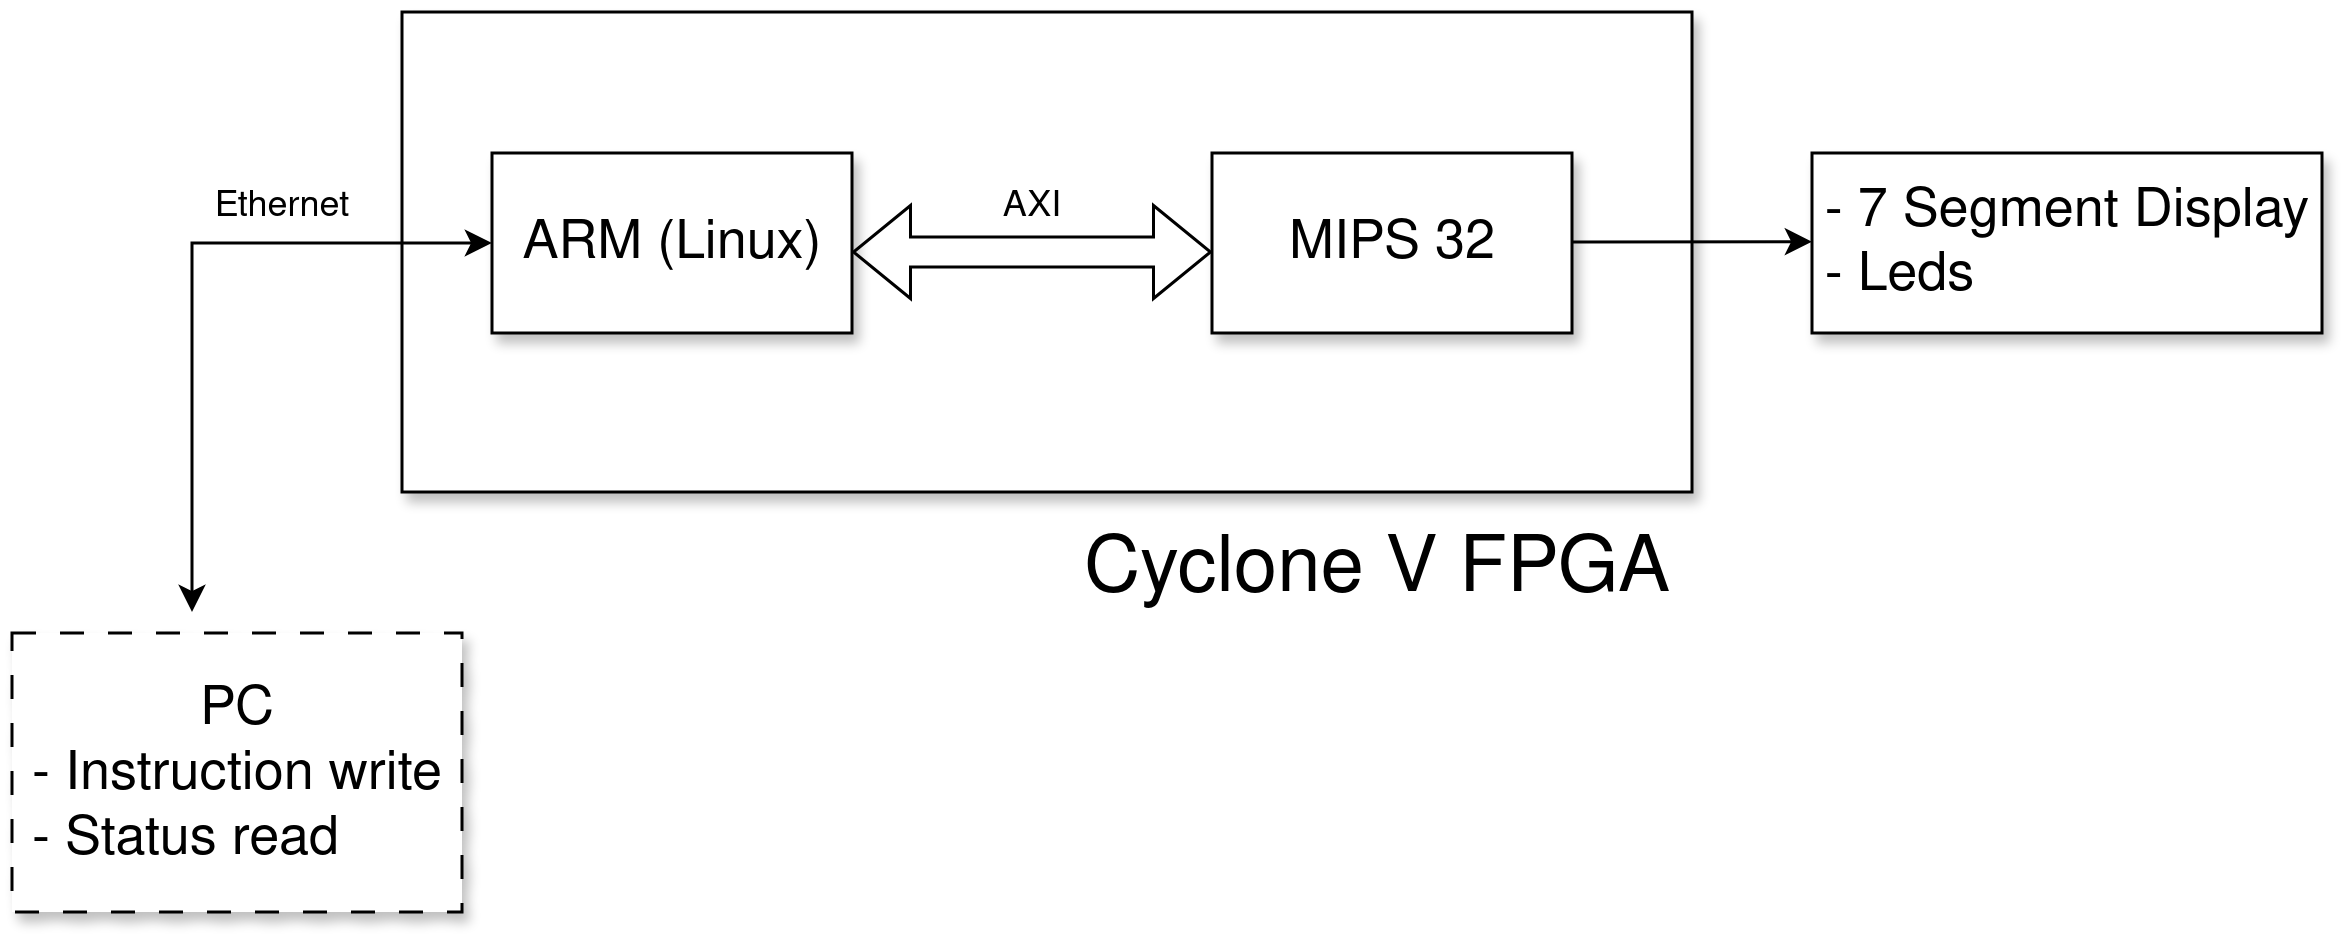
\includegraphics[width=.9\linewidth]{./images/block_diagram.png}
\end{center}

\begin{itemize}
\item FPGA side: MIPS core, instruction memory, data memory, observability logic.
\item HPS side: program loading, state readback, LCD monitor.
\item Result: a complete HW/SW co-design around the processor.
\end{itemize}
\section*{Architecture}
\label{sec:orgefd75e6}
\subsection*{Target vs Implemented Organization}
\label{sec:org74825a0}
\begin{center}
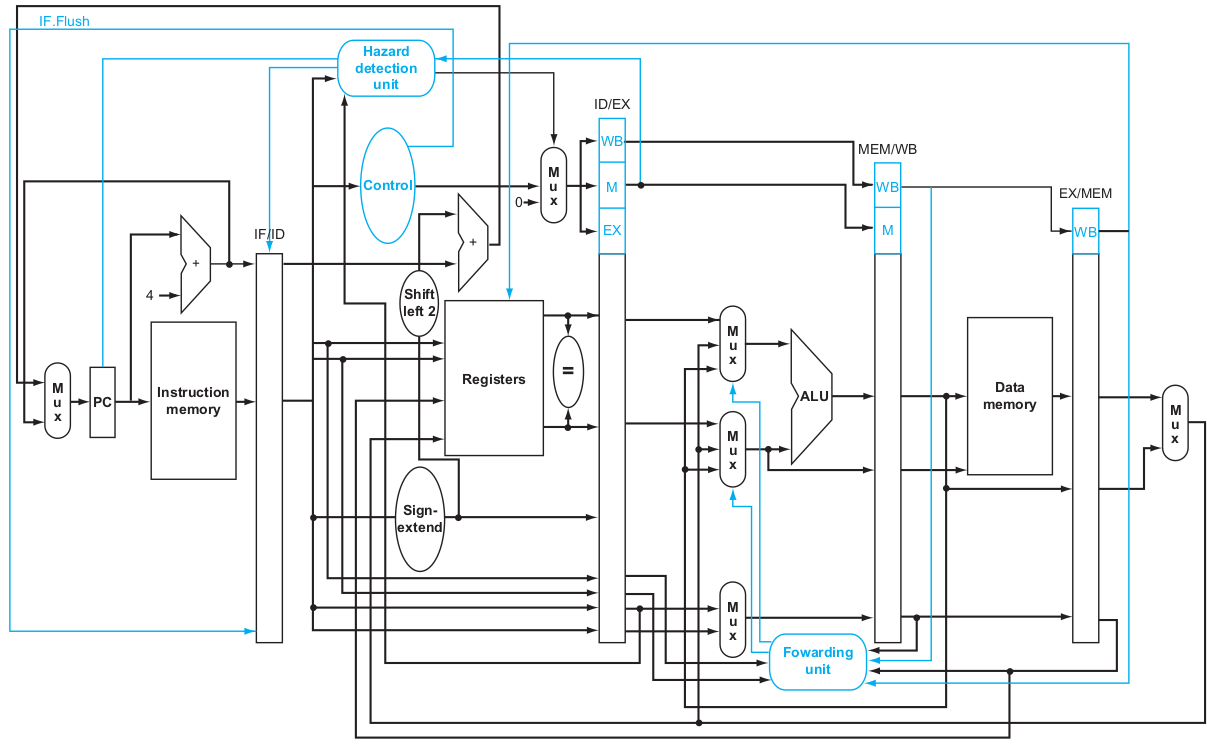
\includegraphics[width=.9\linewidth]{./images/mips.png}
\end{center}

\begin{itemize}
\item The reference starting point is the \emph{classical single-cycle MIPS datapath}.
\item The final implementation is \emph{not a five-stage overlapped pipeline}.
\item Because the Cyclone V BRAMs are synchronous, the design was reorganized into \emph{three execution stages}:
\begin{enumerate}
\item \emph{Fetch}
\item \emph{Execute}
\item \emph{Write-back}
\end{enumerate}
\item Therefore, one instruction completes in \emph{3 clock cycles} in the delivered system.
\end{itemize}
\subsection*{Implemented Processor}
\label{sec:org9f08933}
\begin{itemize}
\item \emph{32-bit datapath} with a \emph{32 x 32-bit register file}.
\item \emph{Harvard organization}: separate instruction and data memories.
\item Main blocks:
\begin{itemize}
\item program counter,
\item register file,
\item main control and ALU control,
\item ALU,
\item sign extension and address-generation logic,
\item BRAM-backed instruction and data memories.
\end{itemize}
\item Supported instruction subset:
\begin{itemize}
\item R-type: \emph{add, sub, and, or, slt}
\item I-type: \emph{addi, lw, sw, beq}
\end{itemize}
\end{itemize}
\subsection*{Why a 3-Stage Execution Model?}
\label{sec:org5ed2827}
\begin{itemize}
\item In the textbook single-cycle view, fetch, decode, execute, memory access, and architectural update all fit in one cycle.
\item On this FPGA, \emph{instruction and data memories are synchronous BRAMs}.
\item This means memory outputs are not immediately available in the same combinational path.
\item The practical solution was to serialize execution into:
\begin{itemize}
\item \emph{Fetch}: read instruction memory,
\item \emph{Execute}: decode, read registers, compute ALU result,
\item \emph{Write-back}: update register file or finalize memory effect.
\end{itemize}
\item This keeps the architecture simple and robust for demonstration.
\end{itemize}
\section*{Platform Integration}
\label{sec:org22b7d4a}
\subsection*{HPS-FPGA Interface and Observability}
\label{sec:orge8287b7}
\begin{itemize}
\item The HPS accesses the processor through the \emph{lightweight HPS-to-FPGA AXI bridge}.
\item This enables Linux user-space tools to:
\begin{itemize}
\item load instruction memory,
\item inspect data memory,
\item read exported status registers.
\end{itemize}
\item Board peripherals are used as debug interfaces:
\begin{itemize}
\item \emph{LCD}: current PC and nearby instructions,
\item \emph{seven-segment displays}: recent stored values,
\item \emph{LEDs}: execution state and control information.
\end{itemize}
\end{itemize}
\subsection*{Demonstrator on the Board}
\label{sec:orgd8e2e11}
\begin{center}
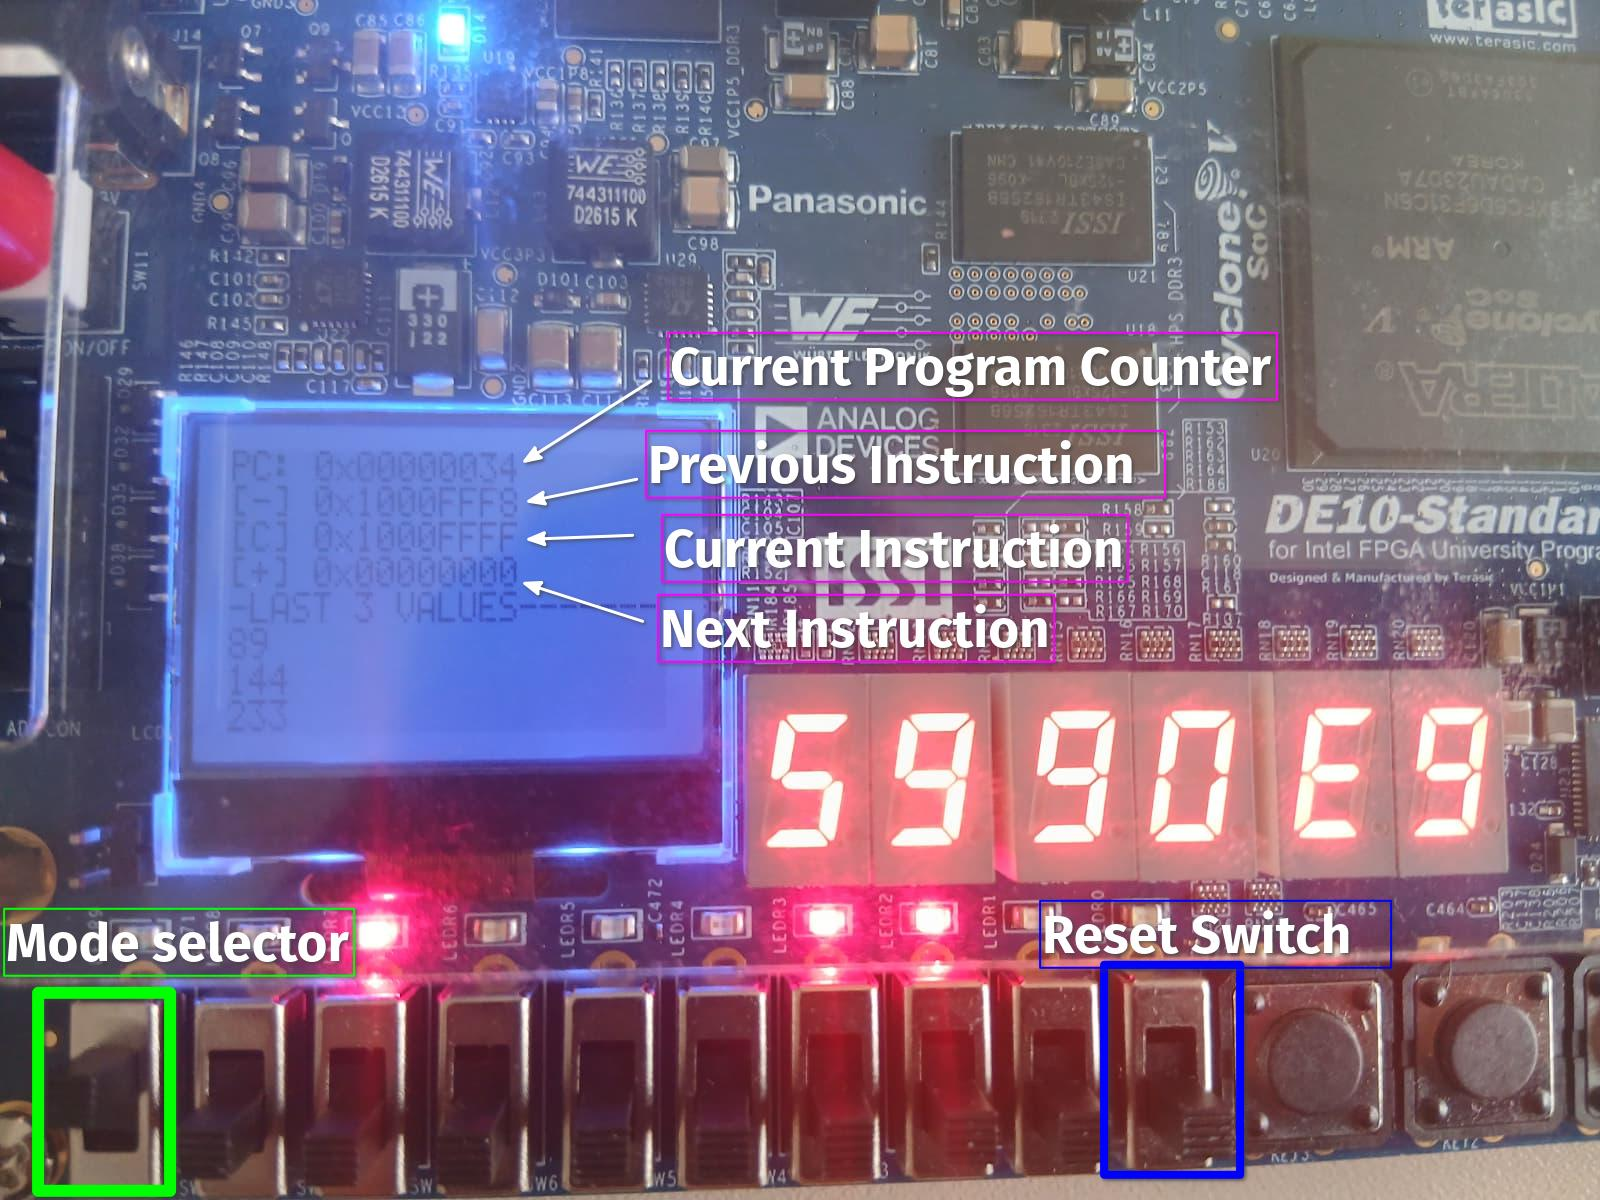
\includegraphics[width=.9\linewidth]{../../report/images/visual.jpeg}
\end{center}

\begin{itemize}
\item \emph{Manual mode}: step through fetch, execute, and write-back.
\item \emph{Automatic mode}: run continuously.
\item The \emph{switcher} block controls when state updates are allowed.
\item A small FIFO keeps the \emph{three latest stored values} for visual observation.
\end{itemize}
\section*{Development}
\label{sec:orgb38ef09}
\subsection*{Development Methodology}
\label{sec:org6dd7509}
\begin{itemize}
\item The project followed a \emph{bottom-up approach}:
\begin{enumerate}
\item validate elementary blocks in simulation,
\item integrate the datapath,
\item connect memories and HPS interfaces,
\item validate the complete system on hardware.
\end{enumerate}
\item Main tools:
\begin{itemize}
\item \emph{VHDL} for RTL,
\item \emph{Quartus} and \emph{Platform Designer} for synthesis and SoC integration,
\item \emph{ModelSim} for unit simulation,
\item \emph{Python} for the assembler,
\item \emph{C} for HPS-side utilities.
\end{itemize}
\end{itemize}
\subsection*{Main Building Blocks Delivered}
\label{sec:orgaf89ca0}
\begin{itemize}
\item \emph{Program counter} with reset and enable.
\item \emph{Register file} with 2 read ports, 1 write port, and hardwired register 0.
\item \emph{Main control} for opcode decoding.
\item \emph{ALU control} and \emph{32-bit ALU}.
\item \emph{Instruction and data BRAMs}.
\item \emph{Switcher} for three-stage execution control.
\item \emph{FIFO and status exports} for observability from the HPS and the board peripherals.
\end{itemize}
\section*{Validation}
\label{sec:org0619a93}
\subsection*{Validation Strategy}
\label{sec:orgf2653b5}
\begin{itemize}
\item \emph{Unit-level validation} in simulation:
\begin{itemize}
\item ALU,
\item ALU control,
\item register file,
\item program counter,
\item main control.
\end{itemize}
\item \emph{Integration validation}:
\begin{itemize}
\item HPS-to-FPGA AXI bridge read/write tests,
\item instruction-memory programming from Linux,
\item data-memory readback.
\end{itemize}
\item \emph{System-level validation}:
\begin{itemize}
\item Fibonacci program,
\item mixed ISA validation program,
\item LCD and seven-segment observation on the board.
\end{itemize}
\end{itemize}
\subsection*{Demo Scenario}
\label{sec:org399eb0f}
\begin{itemize}
\item Assemble the program with the custom Python assembler.
\item Load the generated machine code into \emph{instruction memory} from the HPS.
\item Run the processor on the FPGA in \emph{manual} or \emph{automatic} mode.
\item Observe:
\begin{itemize}
\item \emph{program flow} on the LCD,
\item \emph{recent memory stores} on the seven-segment displays,
\item \emph{memory contents} through HPS-side utilities.
\end{itemize}
\item This validates the entire chain from assembly source to hardware execution.
\end{itemize}
\subsection*{Fibonacci Demonstration}
\label{sec:org97a50a5}
\begin{itemize}
\item The main demonstrator stores successive Fibonacci values into data memory.
\item Why this program is useful:
\begin{itemize}
\item repeated arithmetic operations,
\item loop control with \emph{beq},
\item repeated \emph{sw} operations,
\item easy numerical verification through memory readback.
\end{itemize}
\item Expected sequence begins with:
\begin{itemize}
\item \emph{0, 1, 1, 2, 3, 5, 8, \ldots{}}
\end{itemize}
\end{itemize}
\subsection*{Demo Evidence}
\label{sec:orgb9358d3}
\begin{center}
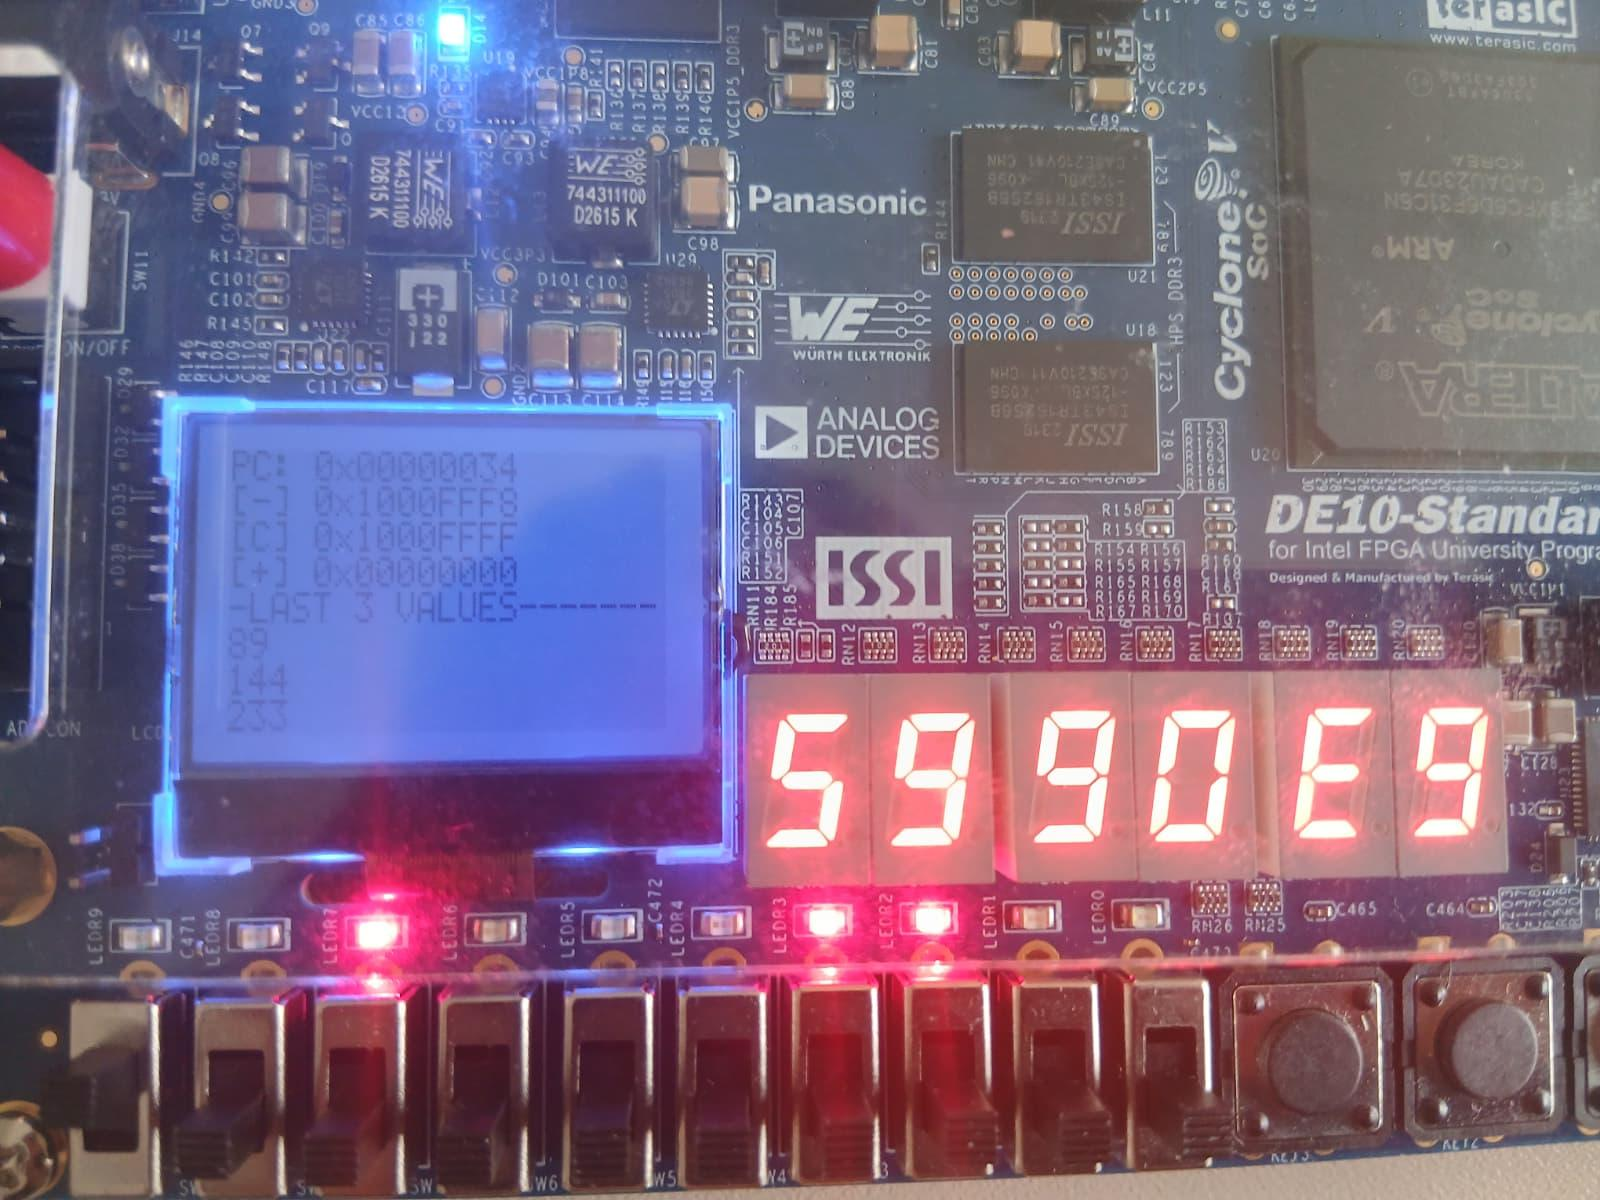
\includegraphics[width=.9\linewidth]{../../report/images/normal_fibo.jpeg}
\end{center}

\begin{center}
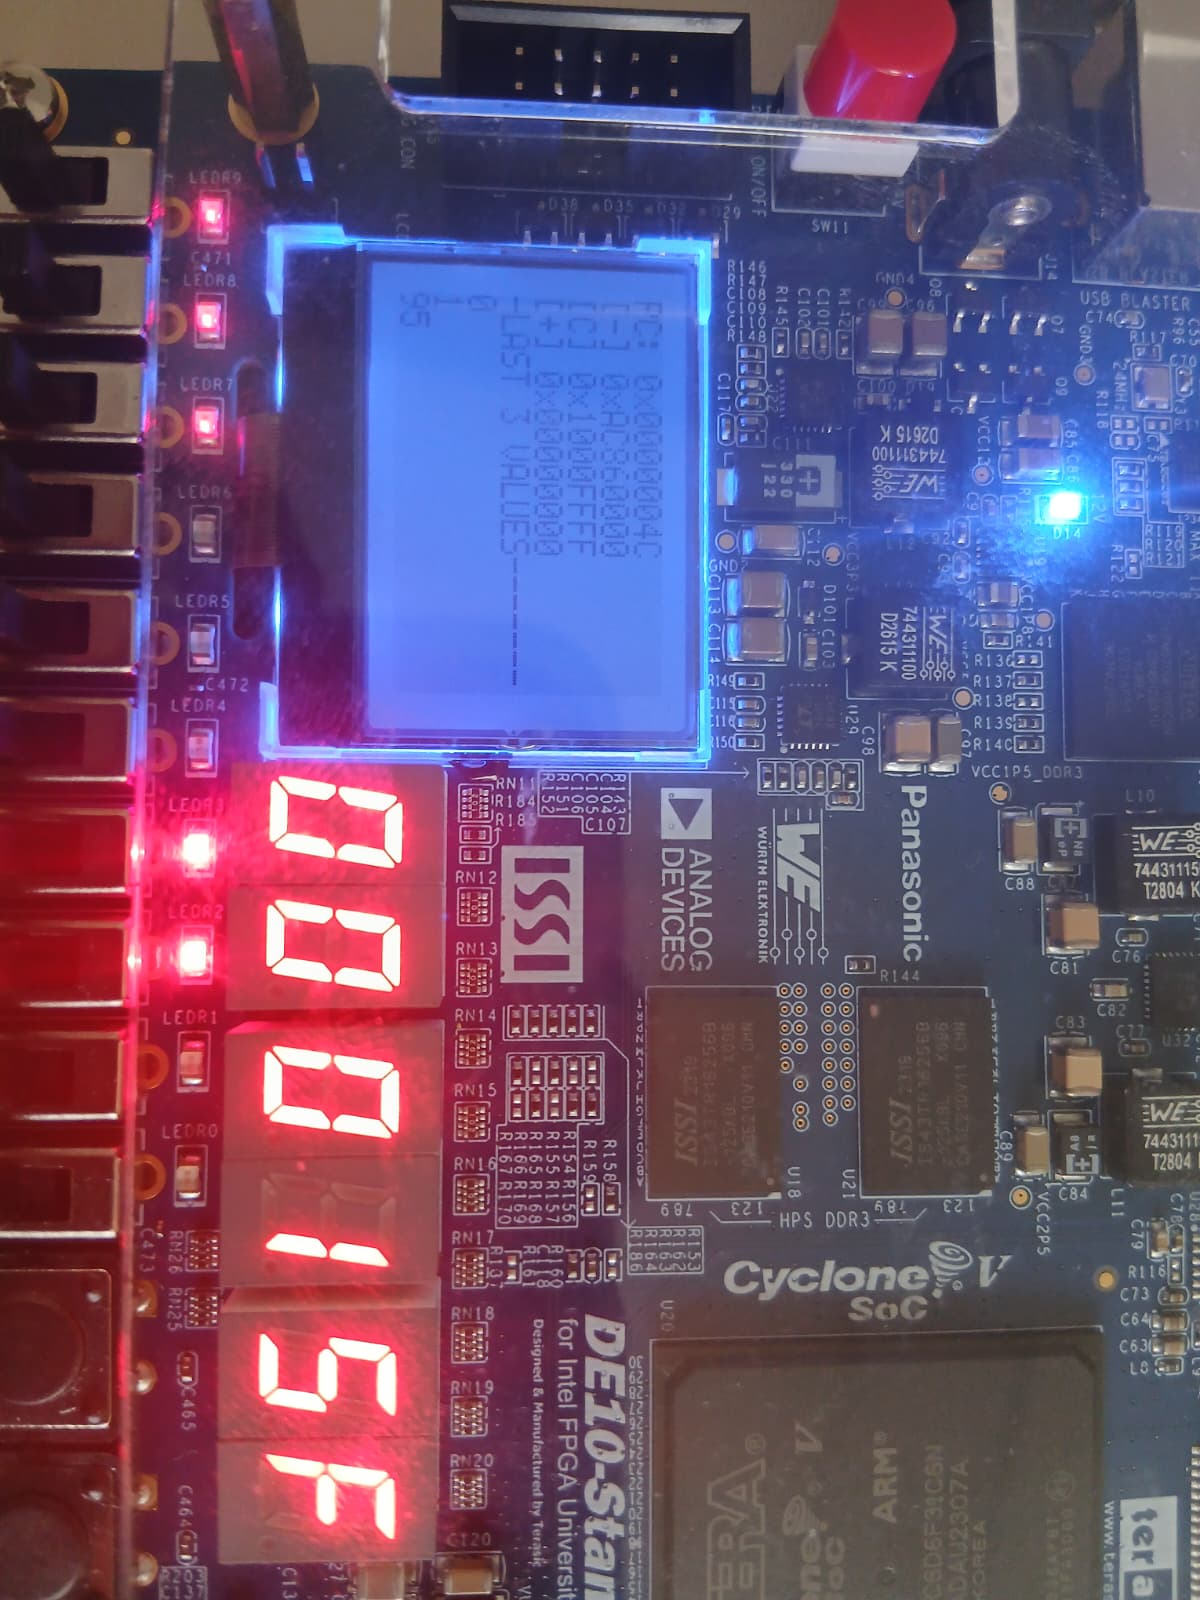
\includegraphics[width=.9\linewidth]{../../report/images/isa.jpeg}
\end{center}

\begin{itemize}
\item Left: Fibonacci execution on the board.
\item Right: separate ISA validation program.
\item These images show that the demonstrator is not limited to one benchmark only.
\end{itemize}
\subsection*{Observed Limitation}
\label{sec:org9604d1f}
\begin{center}
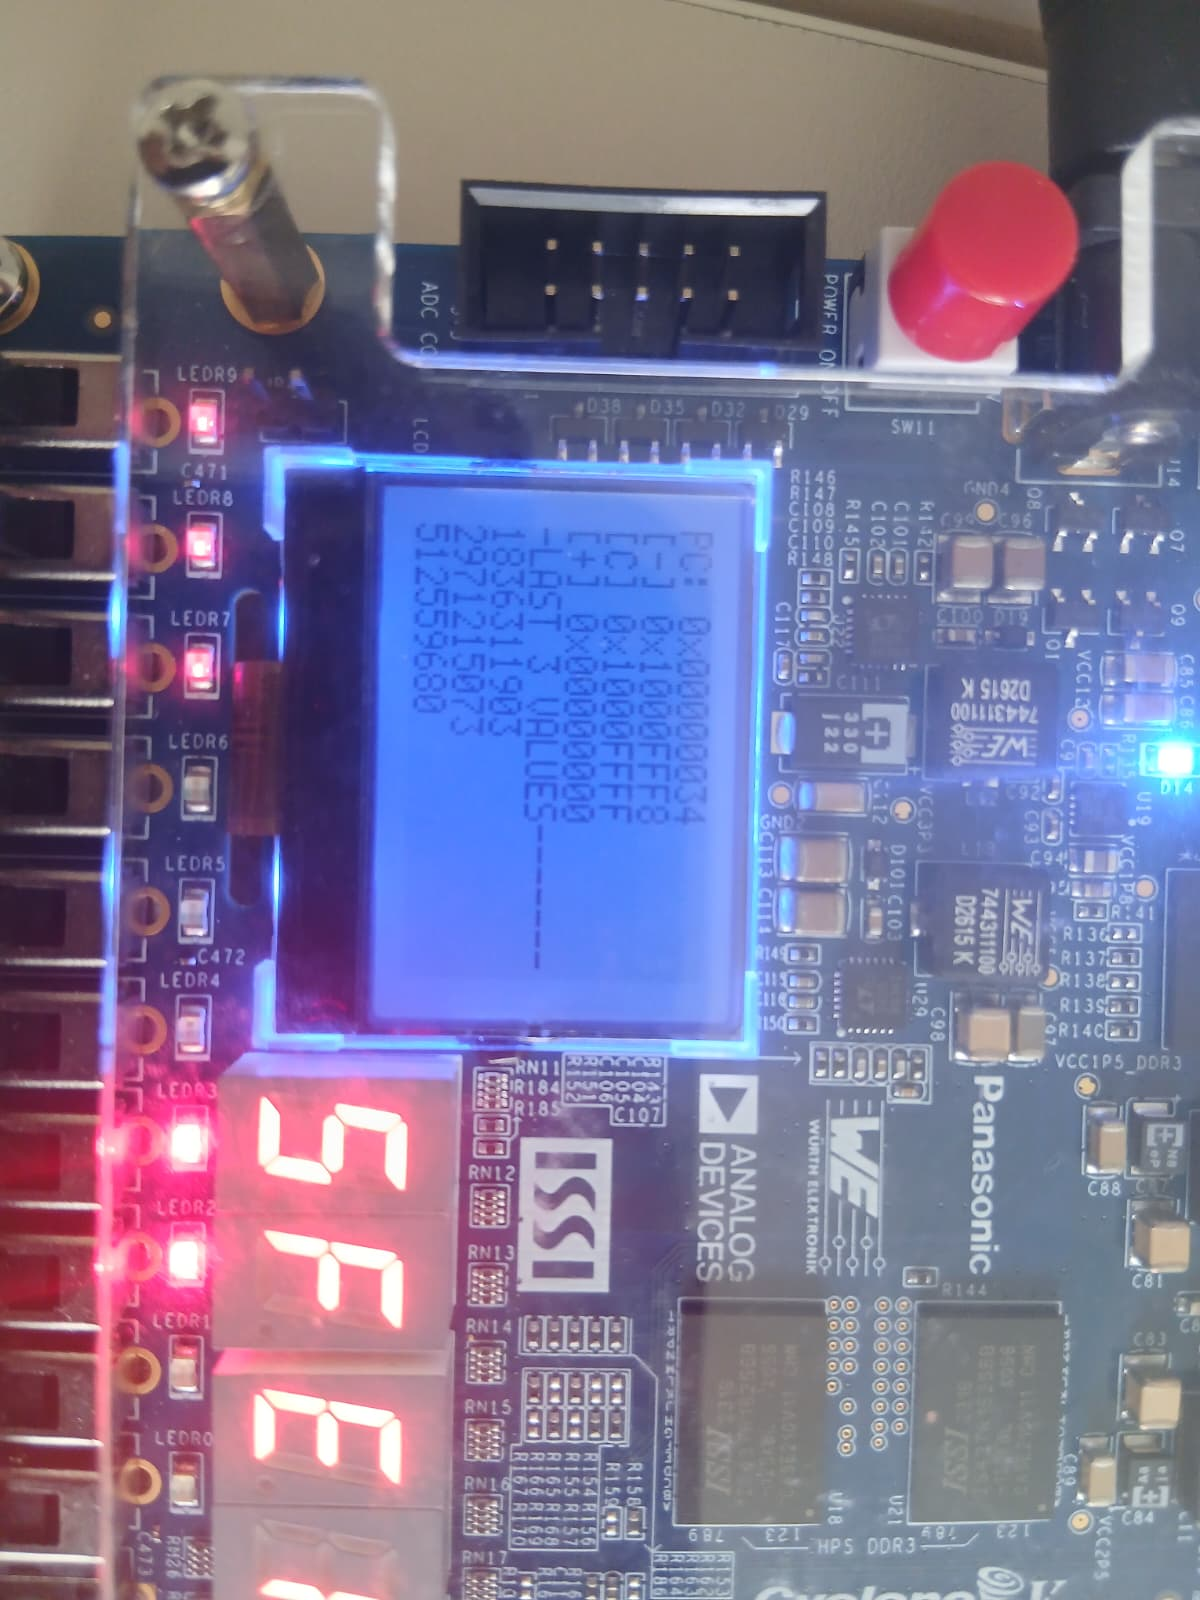
\includegraphics[width=.9\linewidth]{../../report/images/32_bit_limit.jpeg}
\end{center}

\begin{itemize}
\item The datapath and register file are \emph{32 bits} wide.
\item Fibonacci eventually exceeds \(2^{32}\).
\item The stored result then \emph{wraps around modulo \(2^{32}\)}.
\item This is not a bug in the demonstrator: it is the expected consequence of a 32-bit implementation.
\end{itemize}
\subsection*{Resource Utilization}
\label{sec:org6814b62}
\begin{itemize}
\item Post-fit utilization on \emph{Cyclone V 5CSXFC6D6F31C6}:
\begin{itemize}
\item \emph{2,000 ALMs} out of \emph{41,910} available, about \emph{5\%},
\item \emph{3,230 registers},
\item \emph{65,536 block memory bits},
\item \emph{8 RAM blocks},
\item \emph{0 DSP blocks}.
\end{itemize}
\item Conclusion: the processor and its observability infrastructure fit comfortably on the target FPGA.
\end{itemize}
\section*{Theoretical Discussion}
\label{sec:orgc896e86}
\subsection*{Why Harvard for a 1-CPI Objective?}
\label{sec:org9321f89}
\begin{itemize}
\item In a \emph{5-stage pipelined MIPS}, instruction fetch and data memory access may be needed in the same cycle.
\item With \emph{one shared memory}, this creates a \emph{structural hazard}.
\item A \emph{Harvard architecture} removes this conflict by separating instruction and data memories.
\item Even though the delivered core is not yet fully pipelined, this design choice is already present and remains the correct one for a future \emph{1-CPI} target.
\end{itemize}
\subsection*{RAW Hazard After \emph{lw}}
\label{sec:orge4192ab}
\begin{itemize}
\item Example:
\begin{minted}[breaklines=true,basicstyle=\footnotesize,numbers=left,fontsize=\scriptsize,xleftmargin=\parindent,numberstyle=\tiny,breakanywhere=true]{asm}
  lw   $t0, 0($t1)
  add  $t2, $t0, $t3
\end{minted}
\item In a classical pipeline, the loaded data becomes available too late for the immediately following instruction.
\item Standard solutions:
\begin{itemize}
\item \emph{forwarding} when possible,
\item \emph{stalling} for the specific \emph{lw-use} case.
\end{itemize}
\item In the delivered processor, execution is \emph{serialized}, so this hazard does not appear in the same way.
\end{itemize}
\subsection*{Branch Delay Slot and Control in VHDL}
\label{sec:orgfa2321d}
\begin{itemize}
\item \emph{Branch delay slot}:
\begin{itemize}
\item historical MIPS feature,
\item important for the originally planned pipelined version,
\item not exposed as a visible architectural contract in the delivered demonstrator.
\end{itemize}
\item \emph{Control generation in one cycle}:
\begin{itemize}
\item the control unit is \emph{combinational logic},
\item opcode and function bits propagate through logic equations,
\item signals settle during the clock period before sequential blocks sample them.
\end{itemize}
\end{itemize}
\section*{Conclusion}
\label{sec:org7ef92d8}
\subsection*{Conclusion}
\label{sec:orgf748fe4}
\begin{itemize}
\item The project produced a \emph{working MIPS32-style processor demonstrator} on Cyclone V.
\item The final contribution is both:
\begin{itemize}
\item a functional processor core,
\item a complete experimentation environment with assembler, flasher, HPS tools, LCD monitor, and board-level observability.
\end{itemize}
\item The implementation is \emph{functionally operational} and \emph{hardware-demonstrated}.
\item The key architectural adaptation was moving from the textbook single-cycle view to a \emph{practical 3-stage execution model} compatible with FPGA memories.
\end{itemize}
\subsection*{Future Work}
\label{sec:org1b6c2a9}
\begin{itemize}
\item Move from staged execution to a \emph{true pipelined architecture}.
\item Add \emph{hazard detection and forwarding}.
\item Extend the ISA, especially jumps and additional immediate operations.
\item Improve performance analysis and timing closure.
\item Strengthen the HPS monitor with richer debug information.
\end{itemize}
\subsection*{Thank You}
\label{sec:org5735b75}
\begin{itemize}
\item Questions?
\item Contact: hanan.quispe-condori@polytechnique.edu
\end{itemize}
\end{document}
